\section{Preliminary Results}
\label{sec-results}

To explore the potential to transform our discarded Nexus~S~4G smartphones
into low-power sensors, the authors divided into two teams and engaged in a
lifetime programming competition. Each team was provided five discarded
Nexus~S~4G phones and given two weeks to write a program that recorded
battery and light levels every 15~minutes and transmitted them to a server
over a Wifi connection. The goal was to implement a sensing application that
would last as long as possible, while maintaining data delivery to the
server. A gap of over two hours in the data values as observed by the other
team rendered the node as dead, regardless of the amount of energy it had
reported, with the two hour delay chosen to represent the potential
requirements of a somewhat delay-tolerant application.

\begin{figure}[t]
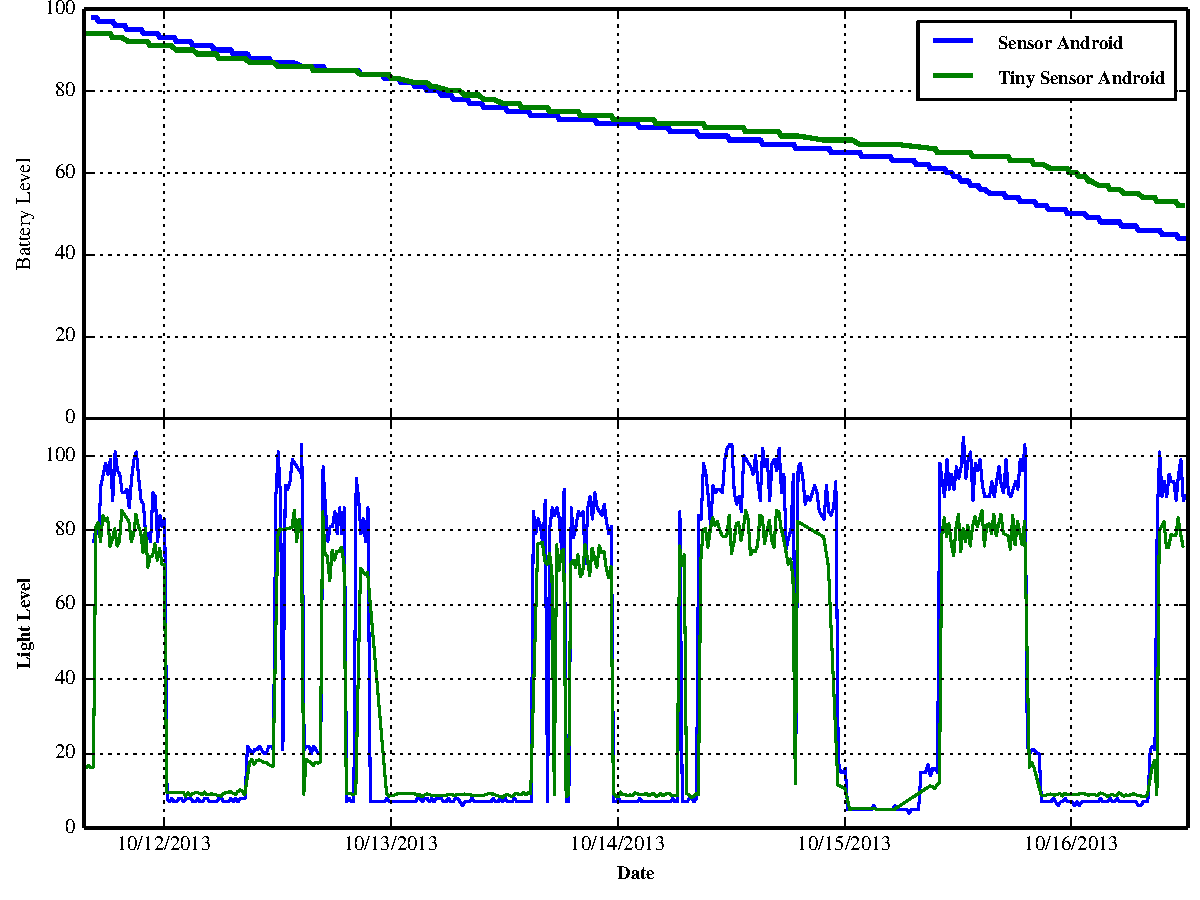
\includegraphics[width=\columnwidth]{./figures/comparison.pdf}

\caption{\small Lifetime results for two light sensing applications.
\textnormal{Both the Tiny Sensor Android (Section~\ref{subsec-tiny}) and
Sensor Android (Section~\ref{subsec-full}) approaches were projected to
achieve a lifetime of 8--9 days.}}

\label{fig-comparison}
\end{figure}


\XXXnote{Overall results.}

Broadly speaking the teams explored two different options with important
implications for reuse in this context: starting with a stock AOSP platform
build and the familiar Android API, or using a super-minimal Tiny Android
build that discards most of the platform components. We refer to the first
approach as ``Sensor Android'' and the second as ``Tiny Sensor Android''.
From a programming perspective, we were hopeful that we could preserve the
familiar Android environment that many programmers today are learning. But
from an energy management perspective, we were worried that the platform
contained features designed around short lifetimes that would prove
unhelpful. We describe both approaches in more detail below.

\subsection{Tiny Sensor Android}
\label{subsec-tiny}

Tiny Android is a development option enabling a stripped-down build intended
for testing new devices, and was not suitable for our application without
modifications. Wifi drivers along with \texttt{dhcpcd} and
\texttt{wpa-supplicant} had to be added to the build process. The only
dependency introduced was \texttt{openssl}. The total package count was
increased by 6, from 11 to 17.

The implementation is primarily in C, consisting of 1500~lines-of-code
(LOC). The program comprises of an infinite loop containing a set of operations. 
First, an alarm is set to wake up for the next sample. Then, the light
sensor is enabled and a sample is obtained from the sensor as well as the
battery. The Wifi interface is then enabled for a short period to send the
message and disabled immediately after. The kernel is then asked to suspend the
device until it is woken up by the alarm.
Measurements showed that each iteration kept the device awake for \XXXnote{?:
period}.

Figure~\ref{fig-tinyandroid} shows current output for one sense-and-send
cycle of our sensing application on Tiny Sensor Android. While the sensing
and transmission complete quickly, allowing the phone to rapidly return to
idle, there was an extra 8~mA of current during the idle state which we have
yet to explain. We believe it may be caused by \XXXnote{GWA : Guru TODO}.

\begin{figure}[t]
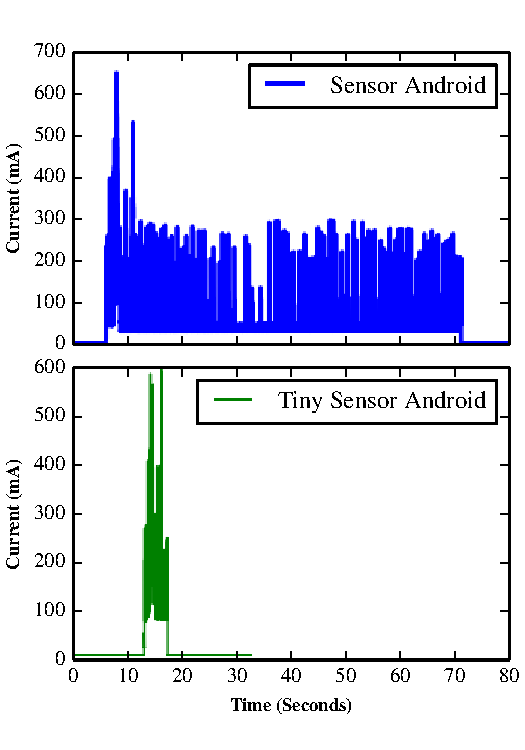
\includegraphics[width=\columnwidth]{./figures/traces.pdf}

\caption{\small Current draw for a single sense-and-send cycle.
\textnormal{Both the Tiny Sensor Android (Section~\ref{subsec-tiny}) and
            Sensor Android (Section~\ref{subsec-full}) have similar current draw for sensing and sending.}}

\label{fig-tinyandroid}
\end{figure}


\subsection{Sensor Android}
\label{subsec-full}

\XXXnote{GWA: Anand TODO} 
The image for the Sensor Android build was built from the latest available AOSP code 
from the JRO03R branch. No changes were made to the platform as we wanted to measure 
the performance of stock AOSP against TINY Android build.
However we manually disabled all the default apps that are part of the stock AOSP build like Browser, 
Calendar, Email, etc. through the settings to disable some of the background services spawned by these applications. 
Although this could have been done in the build scripts of the platform, 
we didn't want to change the stock platform to keep the application development process as simple as possible.

The sensing application was written in 291 LOC using the API's provided by the Android framework. 
Before the start of the experiment, we assigned a static IP to the Wifi interface and the phone was put into airplane mode to 
disable the cellular radio interface, Android allows users to use other radios like the Wifi to be enabled in airplane mode.
The sensing application controlled the enabling and disabling of the Wifi radio interface for each sensing period.

Figure~\ref{fig-tinyandroid} shows the current output for one sense-and-send cycle of our 
sensing application on the Sensor Android. Our sensing application completes the sense and 
send cycle quickly comparable to Tiny Sensor. This is seen in the initial high current draw period 
in the graph, however we notice that there is a 60 second long tail before
the phone goes into the idle state. On further investigation, we found that the 
~\textit{ConnectivityService} in the Android framework holds a ~\textit{Wakelock} for 60 seconds to allow other 
radio interfaces to connect  to a network after one of the interfaces is disconnected. 
For our sensing application this is not required and the platform code can be easily modified to disable this behavior.

\subsection{Expected Lifetime}
Smartphones come with high capacity batteries to power the various components of the smartphone and enable it to be used for a reasonable amount of time by the user before it is recharged. Given the fact that we are not using most of the power hungry components like the Display, GPS, etc. in our sensing application, we expect to see a long lifetime for our application on a fully charged battery. Based on the power measurements conducted for each of the three phases of the application \textit{Idle}, \textit{Sense} and \textit{Transmit} we model the expected lifetime achievable for a sensing application in Equation ~\ref{label_exptime} 
\begin{equation}\label{label_exptime}
    E(T)_{hrs} = \frac{C_{Batt}}{I_{idle} + s*I_{sense}}
\end{equation}
where:
{\small
\begin{itemize}[label=]
    \item $E(T)_{hrs}$: Expected time in hours.
    \item $C_{Batt}$: Capacity of the battery in mAH.
    \item $I_{idle}$: Idle current draw in mA.
    \item $I_{sense}$: Sensing and transmit current draw in mA.
    \item $s$: hourly sensing rate.
\end{itemize}
}

The average current draw values measured in our experiments were $I_{idle}=1.56mA$, $I_{sense}=84.06$\footnote{The value excludes the current draw in the observed long tail.} over a period of 5.3 seconds. With a 1500mAH battery and a sensing rate of every 15 minutes, the expected lifetime for our sensing application would be 426.13 Hours. This translates to approximately 18 days of application lifetime. Considering the non linear discharge rate of the battery as seen in Figure~\ref{fig-comparison}, the expected life would be less than the calculated value.


%%\renewcommand{\arraystretch}{1.2}
\begin{table}[h]
        {\footnotesize
            \begin{tabularx}{\textwidth}{rll}

                %\multicolumn{1}{c}{\textbf{Phase}} &
                %\multicolumn{1}{c}{\textbf{Current Draw (mA)}} \\ 
                \textbf{Phase} &
                \textbf{Current Draw (mA)} & \textbf{Time required (S)}\\ 
                %\hline

                Idle & 1.56 & NA\\ 
                Sense & 342.36 & 1.08\\
                Transmit & 414.03 & 5.03\\
                Combined & 1.56 & TODO\\


            \end{tabularx}
        }

        \vspace{-0.1in}

        \caption{Current draw for different phases for the sensing application.}

        \vspace{0.1in}
        %\hrule
        \vspace{-0.2in}

    \label{table-currentdraw}
\end{table}


\subsection{Discussion}

\XXXnote{GWA: TODO: Compare the merits of each approach.}

\XXXnote{GWA: TODO: Future work to automate the AOSP shutdown process,
uninstall unneeded apps, remove unnecessary services, otherwise tune platform
for single-app use.}

\XXXnote{GWA: TODO: Discuss Android on other hardware, reason for 1~mA sleep
current draw (probably memory).}
